\chapter{Trigonometria}

\section{Triângulo retângulo}
%
  Considere o triângulo retângulo, (triângulo que possui um de seus ângulos internos medindo $90 \degree$), como na figura abaixo:
  \begin{figure}[H]
   \centering
   \fbox{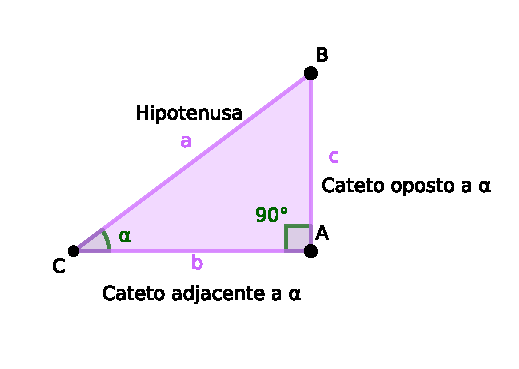
\includegraphics[width=7cm]{Capitulos/Figuras/triangulo_retangulo.pdf}}
   \caption{Triângulo retângulo}
  \end{figure}
 para este triângulo temos que é válido o seguinte teorema:

 \vskip0.3cm

\colorbox{azul}{
 \begin{minipage}{0.9\linewidth}
 \begin{center}
 \textbf{Teorema de Pitágoras}
  \[a^2= b^2 + c^2.\]
 \end{center}
 \end{minipage}}

 \vskip0.3cm

 Este é um resultado importante, já que com ele é possível encontrar o valor de um dos lados do triângulo, nos casos em que não temos todos os lados dados, normalmente é utilizado para encontrar o valor da altura de um triângulo.

 Para este triângulo, as funções seno, cosseno e tangente são dadas pelas seguintes razões trigonométricas, nesta ordem:

 \vskip0.3cm

\colorbox{azul}{
 \begin{minipage}{0.9\linewidth}
 \begin{center}
 \textbf{Funções trigonométricas}
  \begin{eqnarray*}
   \sen(\alpha)= \frac{c}{a}= \frac{CO}{HI} \; \ \
   \cos(\alpha)= \frac{b}{a}= \frac{CA}{HI} \; \ \
   \tan(\alpha)= \frac{c}{b}= \frac{CO}{CA}.
 \end{eqnarray*}
 \end{center}
 \end{minipage}}

 \vskip0.3cm

 Como a soma dos ângulos internos de um triângulo é $180 \degree$, e estamos aqui tratando de um triângulo retângulo, decorre que neste caso $0 \degree \leqslant \alpha \leqslant 90 \degree$. Porém estas funções estão definidas para qualquer número real, mas para nosso estudo é suficiente conhecer seus valores para os ângulos $0 \degree \leqslant \alpha \leqslant 360 \degree$.

 Destacamos aqui os valores do seno, cosseno e tangente dos \emph{ângulos notáveis} que são os mais utilizados:

 \begin{table}[H]
 \centering
 \begin{tabular}{|c|c|c|c|c|c|} \hline
 \rowcolor{cinza}
               & $0 \degree$  & $30 \degree$  & $45 \degree$  & $60 \degree$ & $90 \degree$  \\\hline
  $\pmb{\sen}$ & $0$ &$\frac{1}{2}$ & $\frac{\sqrt{2}}{2}$ & $\frac{\sqrt{3}}{2}$ & $1$ \\\hline
  $\pmb{\cos}$ & $1$ & $\frac{\sqrt{3}}{2}$ & $\frac{\sqrt{2}}{2}$ & $\frac{1}{2}$ & $0$ \\\hline
  $\pmb{\tan}$ & $0$ & $\frac{\sqrt{3}}{3}$ & $1$ & $\sqrt{3}$ & $\nexists$ \\\hline
 \end{tabular}
\end{table}
 Na próxima seção veremos como utilizar estes valores para calcular seno, cosseno e tangente de ângulos maiores que $90 \degree$.

\section{Círculo Trigonométrico}

 No plano cartesiano, consideremos um círculo de centro na origem e raio $1$, neste círculo representamos as imagens das funções trigonométricas aplicadas à  $0 \degree \leqslant \alpha \leqslant 360 \degree$. Como mostra a seguinte figura:
 \begin{figure}[H]
   \centering
   \fbox{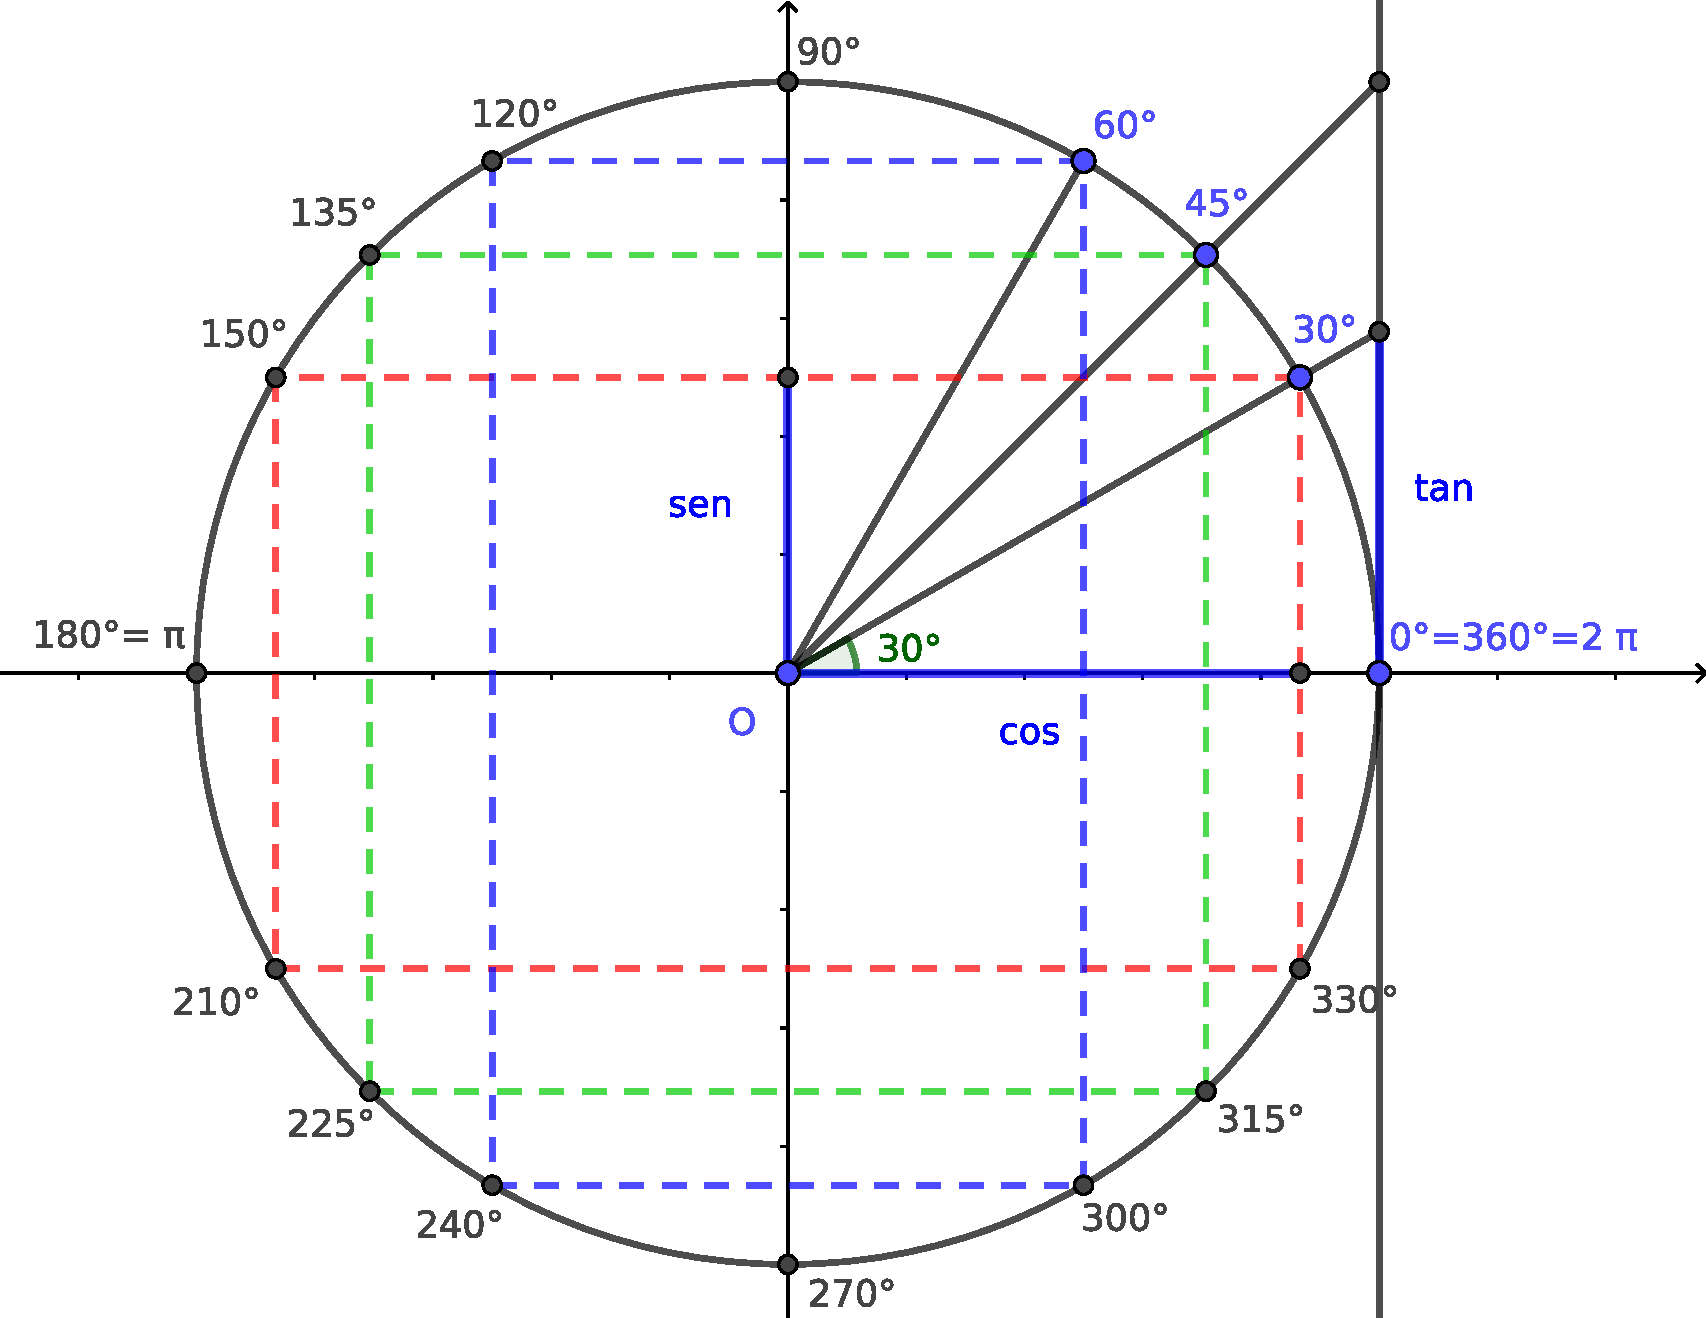
\includegraphics[width=9cm]{Capitulos/Figuras/circulo_trigonometrico.pdf}}
   \caption{Círculo trigonométrico}
  \end{figure}

  A partir do círculo trigonométrico concluímos que:

  \begin{table}[H]
 \centering
 \begin{tabular}{|c|c|c|c|} \hline
 \rowcolor{cinza}
               &  $120\degree$  & $135\degree$  &  $150\degree$ \\\hline
  $\pmb{\sen}$ & $\sen(60\degree)$ &$\sen(45\degree)$ & $\sen(30\degree)$  \\\hline
  $\pmb{\cos}$ & $-\cos(60\degree)$ &$-\cos(45\degree)$ & $-\cos(30\degree)$  \\\hline
  $\pmb{\tan}$ & $-\tan(60\degree)$ &$-\tan(45\degree)$ & $-\tan(30\degree)$  \\\hline
 \end{tabular}
\end{table}

 \begin{table}[H]
 \centering
 \begin{tabular}{|c|c|c|c|} \hline
 \rowcolor{cinza}
                & $210\degree$ & $225\degree$  & $240\degree$  \\\hline
  $\pmb{\sen}$ &  $-\sen(30\degree)$ & $-\sen(45\degree)$ & $-\sen(60\degree)$  \\\hline
  $\pmb{\cos}$ &  $-\cos(30\degree)$ & $-\cos(45\degree)$ & $-\cos(60\degree)$  \\\hline
  $\pmb{\tan}$ &  $\tan(30\degree)$ & $\tan(45\degree)$ & $\tan(60\degree)$   \\\hline
 \end{tabular}
\end{table}

 \begin{table}[h]
 \centering
 \begin{tabular}{|c|c|c|c|} \hline
 \rowcolor{cinza}
               & $300\degree$ & $315\degree$ & $330\degree$ \\\hline
  $\pmb{\sen}$ & $\sen(60\degree)$ & $\sen(45\degree)$ & $\sen(30\degree)$ \\\hline
  $\pmb{\cos}$ & $\cos(60\degree)$ & $\cos(45\degree)$ & $\cos(30\degree)$  \\\hline
  $\pmb{\tan}$ & $-\tan(60\degree)$ & $-\tan(45\degree)$ & $-\tan(30\degree)$  \\\hline
 \end{tabular}
\end{table}


  Os ângulos podem também ser representados em radianos, respeitando a seguinte relação:

  \[\destaque{\pi \text{ radianos}= 180 \degree}\]

  Usando esta relação podemos transformar graus para radianos e radianos para graus, vamos ver dois exemplos:

  \begin{exem}
   Qual a medida em graus do ângulo que mede $\frac{\pi}{4} rad$?

   \underline{Resolução:}

   Sabemos que $\pi rad= 180\degree$, portanto usando a regra de 3 abaixo conseguimos encontrar o valor em graus deste ângulo:
   \begin{eqnarray*}
  \text{Graus} & & \text{Radianos} \\
   180 & = & \pi\\
  x & = & \frac{\pi}{4}
 \end{eqnarray*}
 usando a propriedade da proporcionalidade, ou seja, multiplicando cruzado temos:

 $180 \cdot \frac{\pi}{4}= \pi \cdot x \Rightarrow \pi \cdot x= \frac{180 \pi}{4} \Rightarrow x= \frac{45 \pi}{\pi} \Rightarrow x= 45\degree$.

 \fim
  \end{exem}

  \begin{exem}
   Qual a medida em radianos do ângulo que mede $30\degree$?

   \underline{Resolução:}

   Sabemos que $\pi rad= 180\degree$, portanto usando a regra de 3 abaixo conseguimos encontrar o valor em graus deste ângulo:
   \begin{eqnarray*}
  \text{Graus} & & \text{Radianos} \\
   180 & = & \pi\\
  30 & = & x
 \end{eqnarray*}
 usando a propriedade da proporcionalidade, ou seja, multiplicando cruzado temos:

 $180 \cdot x= \pi \cdot 30 \Rightarrow x= \frac{30 \pi}{180} \Rightarrow x= \frac{\pi}{6} rad$.

 \fim
  \end{exem}



 \section{Relações trigonométricas}

 Só a critério de conhecimento, segue uma lista de algumas relações trigonométricas que são interessantes pela grande quantidade de aplicações:

 \begin{eqnarray*}
  \tan(x)&=&\frac{\sen(x)}{\cos(x)} \\
  \sen^2(x) + \cos^2(x)&=&1 \\
  \sen(a+b)&=&\sen(a)\cdot \cos(b)+\sen(b)\cdot \cos(a) \\
  \sen(a-b)&=&\sen(a)\cdot \cos(b)-\sen(b)\cdot \cos(a) \\
  \cos(a+b)&=&\cos(a)\cdot \cos(b)-\sen(a)\cdot \sen(b) \\
  \cos(a-b)&=&\cos(a)\cdot \cos(b)+\sen(a)\cdot \sen(b) \\
  \tan(a+b)&=& \frac{\tan(a)+\tan(b)}{1-\tan(a)\cdot \tan(b)} \\
  \tan(a-b)&=& \frac{\tan(a)-\tan(b)}{1-\tan(a)\cdot \tan(b)}
 \end{eqnarray*}
 
 \section{Exercícios}
 \begin{exer}
 (Sociesc - 2009) Um grupo de escoteiros foi acampar. Do acampamento avistaram o pico de um morro segundo um ângulo de $30 \degree$. Ao caminharem mais 30 metros em direção ao morro passaram a ver o pico segundo um ângulo de $60 \degree$. Sendo $\sen 30\degree = \frac{1}{2}$, $\cos 30\degree =\frac{\sqrt{3}}{2}$, $\sen 60\degree =\frac{\sqrt{3}}{2}$, $\cos 60\degree =\frac{1}{2}$, $tg 60\degree = \sqrt{3}$ e $tg 30\degree =\frac{\sqrt{3}}{3}$ , altura do morro é:
 \begin{multicols}{2}

 \begin{enumerate}
  \item 15 metros
  \item $\frac{30}{\sqrt{3}-1}$ metros
  \item $\frac{30\sqrt{3}}{1-\sqrt{3}}$ metros
  \item $15\sqrt{3}$ metros
 \end{enumerate}

 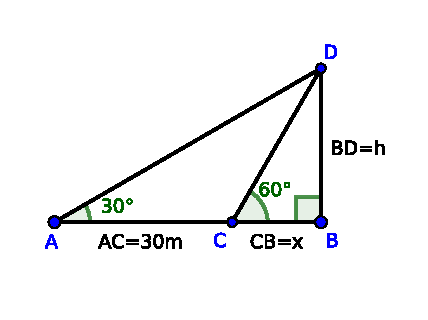
\includegraphics[width=6cm]{Capitulos/Figuras/tri_ret_exer.pdf}

 \end{multicols}
 \end{exer}
 
 \begin{exer}
 (Sociesc - 2010) Uma rampa lisa de 24 m de comprimento faz ângulo de $60\degree$ com o plano horizontal. Uma pessoa que sobe essa rampa inteira atinge o ponto mais alto verticalmente de:

  Dados: $\sen (60\degree)= \frac{\sqrt{3}}{2}$, $\cos (60\degree)= \frac{1}{2}$, $\tan (60\degree)= \sqrt{3}$
 \begin{multicols}{2}

 \begin{enumerate}
  \item $\frac{17 \sqrt{3}}{2} m$
  \item $15\sqrt{3} m$
  \item $12\sqrt{3} m$
  \item $\frac{25 \sqrt{3}}{2} m$
  \item $18\sqrt{3} m$
 \end{enumerate}

 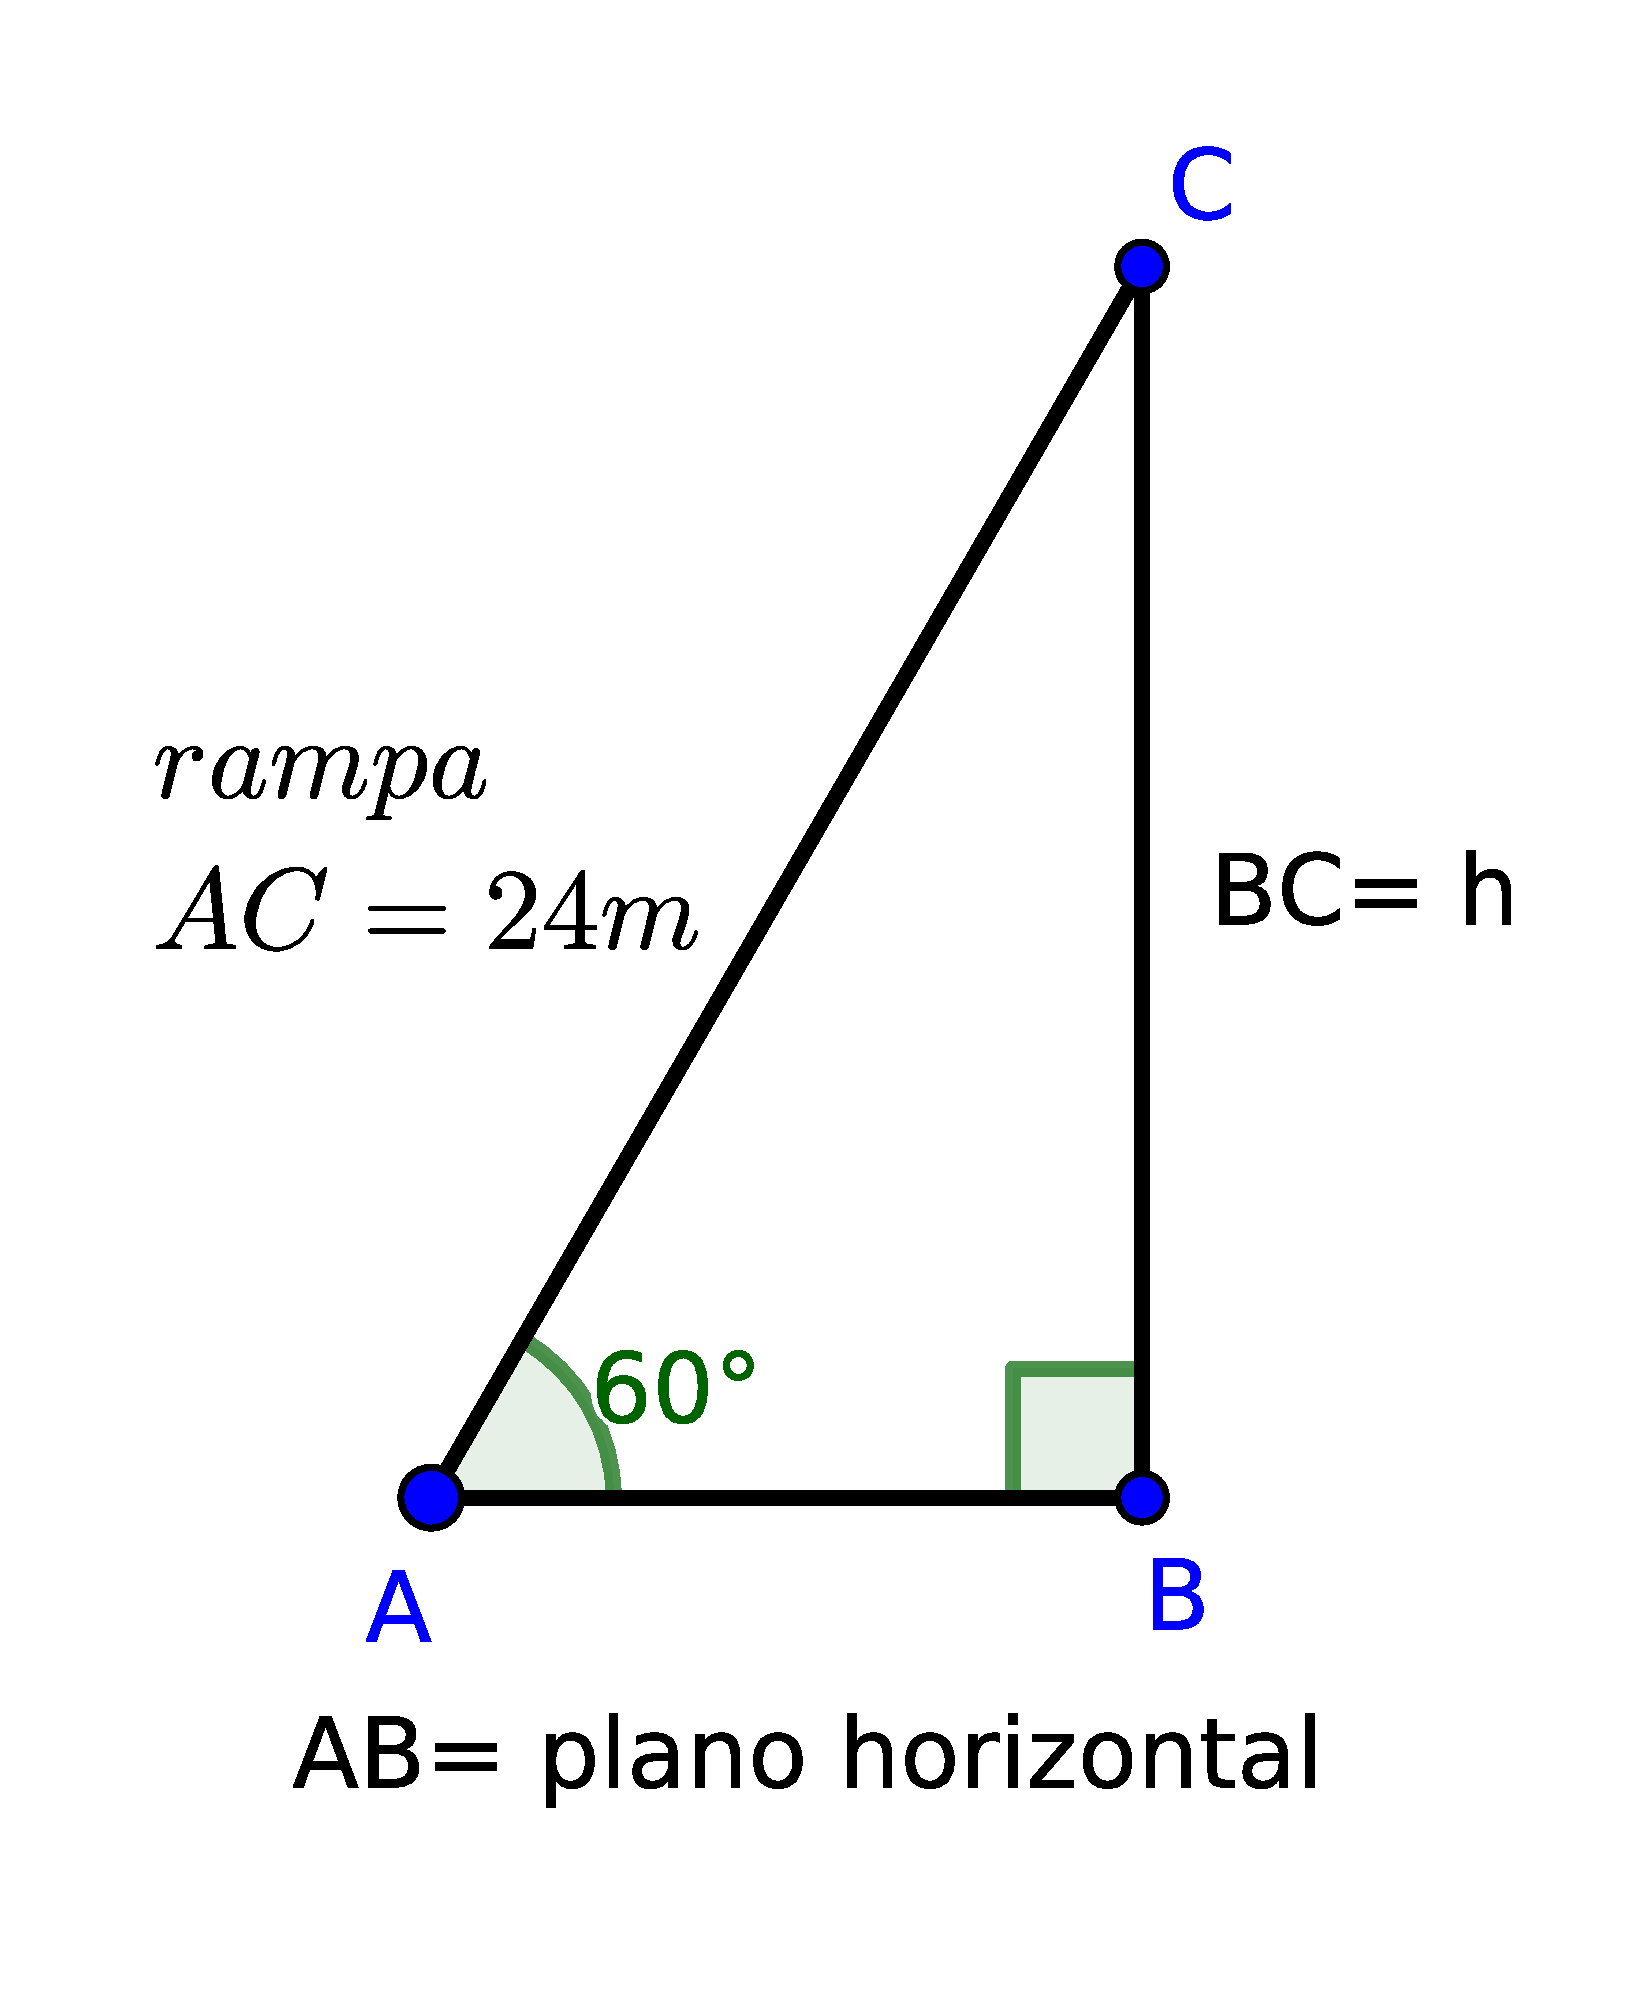
\includegraphics[width=4cm]{Capitulos/Figuras/tri_ret_exer2.pdf}
 \end{multicols}
 \end{exer}
 
 \begin{exer}
 (Sociesc - 2010) Um teleférico deve unir os topos A e B de dois morros. Para calcular a quantidade de cabo necessário foi preciso medir a altura dos morros em relação a um plano horizontal, obtendo-se 108m e 144m respectivamente. A seguir, mediu-se o ângulo que a reta $\overline{AB}$ forma com a horizontal, obtendo-se $32\degree$. Calcule a distância entre os pontos A e B, sabendo que $\sen (32\degree)= 0,52$, $\cos (32\degree)= 0,84$ e $\tan (32\degree)= 0,62$.

 \begin{multicols}{2}

 \begin{enumerate}
  \item 18,72 m
  \item 48,23 m
  \item 69,23 m
  \item 78,45 m
 \end{enumerate}

 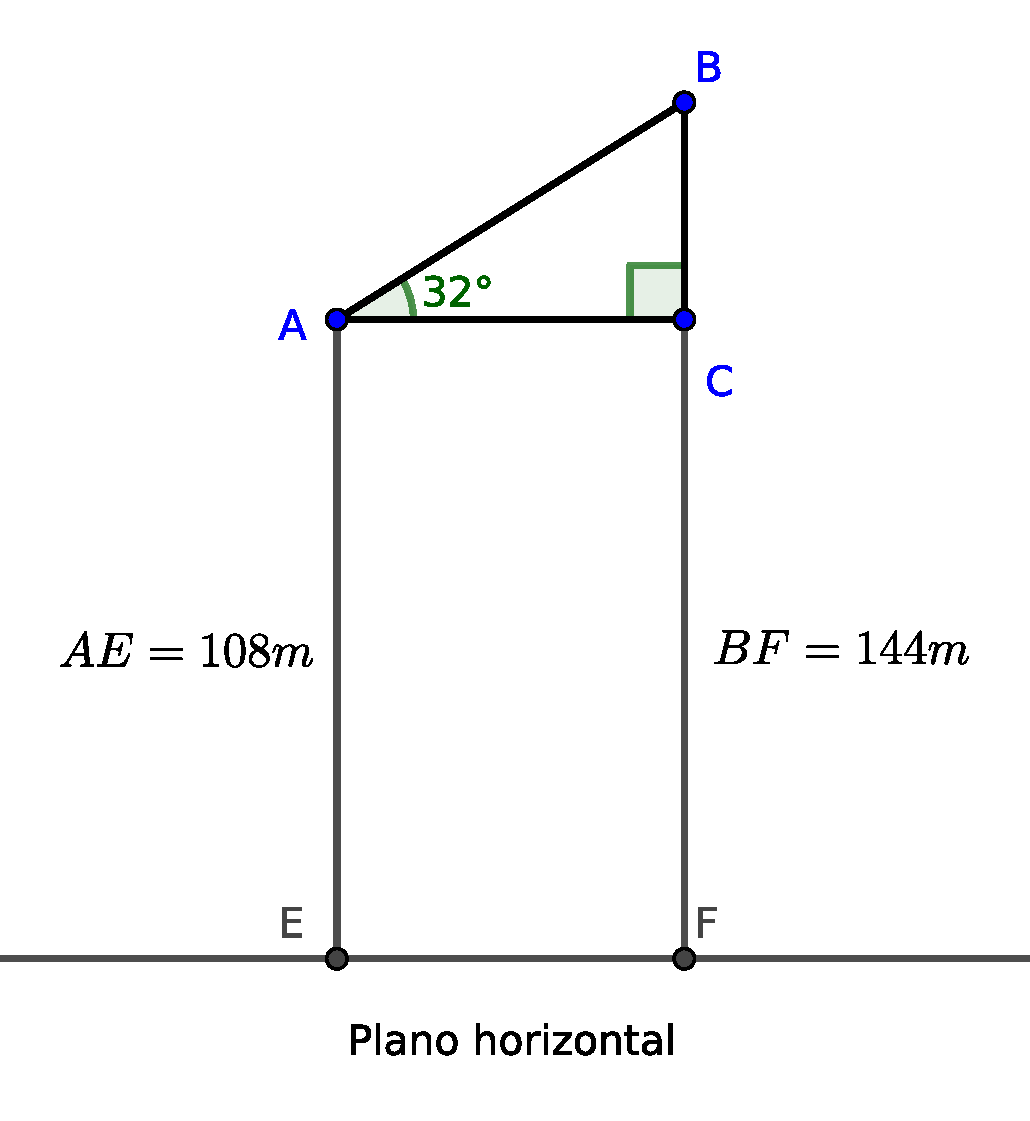
\includegraphics[width=5cm]{Capitulos/Figuras/tri_ret_exer3.pdf}

 \end{multicols}
 \end{exer}
 
 \begin{exer}
 (Sociesc - 2010) No retângulo abaixo retirou-se dos cantos quatro triângulos retângulos sombreados, formando assim um hexágono regular de lado 4cm.
  \begin{figure}[H]
   \centering
   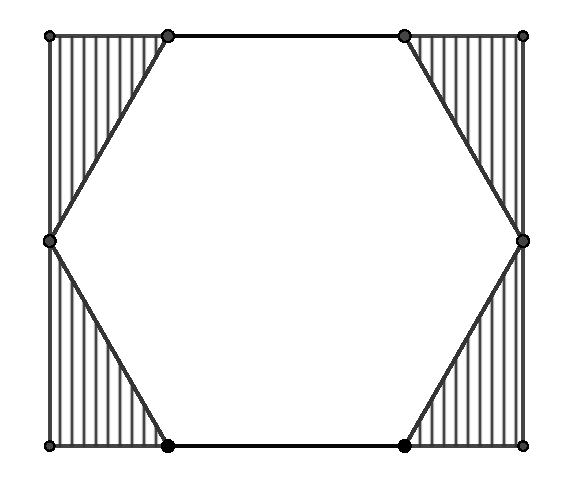
\includegraphics[width=5cm]{Capitulos/Figuras/Hexagono.pdf}
  \end{figure}

  A área do retângulo é:
  \begin{enumerate}
  \item $64cm^2$
  \item $12\sqrt{3}cm^2$
  \item $48cm^2$
  \item $32\sqrt{3}cm^2$
 \end{enumerate}
 \end{exer}

Gabarito: 1 d); 2 c); 3 c); 4 d).

 {\color{red} Nota:} cada ângulo interno de um hexágono mede $120\degree$.
 Pois,
 \vskip0.3cm
\colorbox{azul}{
 \begin{minipage}{0.9\linewidth}
 \begin{center}
 A soma dos ângulos internos de um polígono regular de $n$ lados é dada por:
  \[S= (n-2)\cdot 180 \degree .\]
 \end{center}
 \end{minipage}}
 \vskip0.3cm
 assim, como o hexágono é um polígono regular de $n= 6$ lados, decorre que a soma de seus ângulos internos é:
 \[S= (6-2)\cdot 180= 4 \cdot 180= 720 \degree\]
 portanto, cada ângulo interno $\alpha$ do hexágono mede:
 \[\alpha= \frac{720}{6}= 120 \degree .\]
